%!TEX root = thesis.tex
\todo{ref til ad hoc construction principle} 
For our first \hl{prototype description} we will dig into the area of shape changing interfaces, SCIs.
We will do this to explore and illustrate the possibilities of creating AHIs based on shape-change.
More specifically we will touch upon a specific approach to constructing SCIs called jamming.
SCIs were introduced in the introduction of this thesis as interfaces that use physical change of shape as input or output.
Jamming is special kind of technique that can be used to control the stiffness of a material which makes it possible to construct objects that can change their surface structure.
What makes SCIs interesting to AHIs is it''s ability to dynamically change the physical properties of an interface element, be it shape, texture, stiffness, position ect.
This change in physicality can then be the offset for a new temporary interaction possibility that is created for the specific situation, where afterwards it can return to it''s initial natural state.
This aspect aligns well with the definition of AHIs that we presented earlier in section \todo{ref to AHI section} 

\todo{procesbeskrivelse - udfordring i prototyping 15 linjer!}

\section{Shape-Changing Interfaces}
\label{ch:jamming:shape-change} 
%!TEX root = ../thesis.tex
\label{ch:jamming:vocabulary}
In chapter~\ref{interfaces:physical_computing} we presented the concept of shape-changing interfaces (SCIs) with \citeauthor{rasmussen2012shape} definition of SCIs as

\begin{quotation}
  \emph{A shape-changing interface uses physical change of shape as input or output. \citep{rasmussen2012shape}} 
\end{quotation}
In this chapter we will expand our vocabulary regarding SCIs based on \citet{coelho2011shape} and \citet{rasmussen2012shape}.
They both provide contributions as to how we can talk about SCIs, how we can group and identify different types of change of shape, how we can identify and describe shape transformations, and most importantly, how and to which purpose we can interact with SCIs.
We will use this vocabulary onwards in our thesis to discuss SCIs, both ours and others.   

\citeauthor{coelho2011shape} presents a grouping which distinguish three types of change of shape: \emph{topological, textural and permeable} transformations.
Topological transformations here being those transformations which adhere to topological equivalence, permeable those which do not and textural transformation stands as a category for it.
Topologically equivalence here means that a form can transform in to another form by a continuously homeomorphic transformation - that is without cutting or gluing either form.
This can be exemplified by the pliable donut that transforms into a coffee mug without breaking homeomorphism as seen in figure~\ref{pliable-mug} 

\begin{figure}[h]
  \centering
  \includegraphics[width=0.9\linewidth]{figures/pliable-donut}
	\caption{The pliable donut momeomorphic transformation, taken from \citep{coelho2011shape}}
   \label{pliable-mug}
\end{figure}   
 
\citeauthor{rasmussen2012shape} suggests a grouping more detailed grouping of shape-changing interfaces by identifying eight types of change of shape, namely: \textit{orientation, form, volume, texture, viscosity, spatiality, adding/subtracting and permeability}.
These eight fit into two groups where the first six are topologically equivalent and the last two are not.
This is in line with what \citeauthor{coelho2011shape}, though texture standing has been moved into the topologically equivalent group. Overall it expands on \citeauthor{coelho2011shape}s work and enables us to identify and discuss form changes in more detailed terms.
The grouping is visualized in figure~\ref{types-of-change}, illustrating the different types of change.

\begin{figure}[h]
  \centering
  \includegraphics[width=0.9\linewidth]{figures/types-of-change}
	\caption{Types of shape-change as visualised by \citep{rasmussen2012shape}}
   \label{types-of-change}
\end{figure}

There might be some debatable cases in this grouping, e.g. they define textural change as
\begin{quotation}
  \emph{small changes on the surface of the shape that add visual and tactile properties without affecting the overall form}
\end{quotation} 
so if the overall form is not changed it might not make sense to classify it as a homomorphic transformation, which might also be the reason why \citeauthor{coelho2011shape} chose to separate it as a case for itself.
Also if we look at the case of spatiality changes where a collection of elements form a single object, it is possible to think of examples where non-homeomorphic transformations occurs if, for example, the collection of elements split in the middle forming two objects and then merge back together.
This would still count as a shape-changing interface as described in the definition but would not adhere to topological equivalence.   

The transformation in itself is interesting as well and \citeauthor{rasmussen2012shape} identify different types of transformation.
They describe the transformation as the \textit{phase between endpoints}, meaning the phase between the form's origin and its morphed state.
They distinguish between kinetic parameters and expressive parameters, where the kinetic parameters describe the physical movements of the transformation and the expressive parameters relate to how the kinetic movements are perceived and understood.
This is a very interesting and important aspect of SCIs since it, together with the theory of affordances, provides the basis for understanding the interface and its functions, which at the same time is one of the key challenges of SCIs.
Since SCIs are inherently non-static objects we might not be able to rely on the form alone to communicate the intent and functions of the object. As a change in form can cause a change in function the initial perceived affordance of an object might not cover all of the interaction possibilities of that object, so there might have to be some interaction clues elsewhere, for example in the transformation itself.

A key aspect of SCIs, and any user interface in general, is the interaction - be it direct physical interaction, implicit visual interaction, or something in between. 
\citeauthor{rasmussen2012shape} distinguish between \textit{no interaction}, where there is only shape-changing output; \textit{indirect interaction}, still only with shape-changing output but based on implicit user input; \textit{direct interaction}, where the user deforms the object in some way as user input and a shape-change output occurs, either in the object itself or in a remote object.
Two approaches to direct interaction are identified, \textit{action and reaction} where the object reacts directly to the action in a synchronized process and \textit{input and output} where the object is acting asynchronously and not necessarily directly related to the input.

In the next session we proceed into the area of jamming, an approach that we see as an interesting enabling technology for SCIs.
Jamming allows for many of the different types of transformations as we will see both in the related jamming applications and in our own concepts. 

Our focus will be on objects with direct interaction and mainly those with input and output merged into the same object, as we here see the best possibilities for creating interfaces \todo{et eller andet}
 
Our own exploratory work will focus only on topological transformations, excluding spatiality, since our choice of technology hinders this type of change. This will be further described in the following section.

\section{Jamming as an enabling technology}
\label{ch:jamming:enabling-technology} 
%!TEX root = ../thesis.tex
Before continuing on the topic of jamming interfaces, let us first give an introduction to the mechanics of jamming.

Jamming is a mechanism that can enable granular material to transition between solid-like and liquid-like states. 
These states are achieved by varying an external stress on the material.
Even though a granular material is not a compound in itself these states show that it resembles the behaviour of a chemical compound such as water, which can shift between vapor, liquid and ice under an external stress such as temperature.
A granular material, such as sand may resemble a liquid as it flows through an hour glass, although the individual grains themselves are a solid structure. 
If this granular material exist within a confined space and are put under an external stress such as pressure, they jam against each other with no ability to escape.
Figure~\ref{fig:ch:jamming:particles:jam_unjam} illustrates the behaviour of granular material in the two states.

\begin{figure}[h]
\centering
\begin{subfigure}[b]{.44\textwidth}
  \centering
  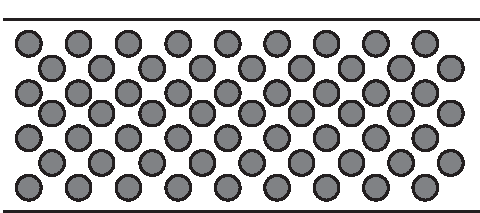
\includegraphics[width=\linewidth]{figures/jamming/particles_unjammed.pdf}
  \caption{Granular material flowing freely in a liquid-like state.}
\end{subfigure}%
\hspace{0.02\textwidth}
\begin{subfigure}[b]{.44\textwidth}
  \centering
  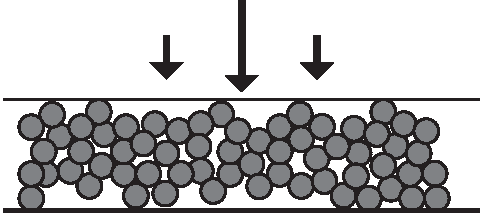
\includegraphics[width=\linewidth]{figures/jamming/particles_jammed.pdf}
  \caption{Granular material jammed in a confined space due to pressure.}
\end{subfigure}
\caption{Different granular material.}
\label{fig:ch:jamming:particles:jam_unjam}
\end{figure}

You might have noticed how some coffee packagings at the local super market are like a rigid container, see figure~\ref{fig:ch:jamming:coffee-packaging}. 
In this kind of packaging, after filling it with coffee, all excess air has been sucked out by applying a vacuum, thereby jamming the coffee grains and making it almost rock solid. 
After opening the packaging the form and viscosity of the structure change instantly as air is let in releasing coffee grains from their jammed state.
Another example is a regular bean bag which exhibits some of the same properties, see figure~\ref{fig:ch:jamming:bean-bag}. 
When no force is applied to it, i.e. no one is sitting in it, it resembles the liquid-like state mentioned earlier. 
Then, when a person sits down in it, air will be pressed out and the particles (most often polystyrene foam) will be pushed tightly together filling voids and thereby jamming the particles making it resemble a solid.

\begin{figure}[h]
\centering
\begin{minipage}[t]{.44\textwidth}
  \centering
  \includegraphics[width=.5\linewidth]{figures/jamming/coffee_packaging}
  \captionof{figure}{Coffee in vacuum packaging.}
  \label{fig:ch:jamming:coffee-packaging}
\end{minipage}%
\hspace{0.02\textwidth}
\begin{minipage}[t]{.44\textwidth}
  \centering
  \includegraphics[width=.5\linewidth]{figures/jamming/bean_bag}
  \captionof{figure}{A bean bag.}
  \label{fig:ch:jamming:bean-bag}
\end{minipage}
\end{figure}

\subsection{Particles}
\label{ch:jamming:particles}
The granular material, also called the particles, can be any material that has the physical properties that allow for jamming to occur. 
But parameters such as particle size, shape and compressibility have an impact on the jamming transition. 
This has been investigated by several researchers, e.g. \cite{cheng2012design} and \cite{steltz2010jamming}, where the stress to strain ratio of different granular materials are evaluated. 
Ground coffee (fine and coarse) and glass beads of varying size are recurring across these tests, the first being an irregular shape with a rough surface as opposed to the plain shape and smooth surface of the second, see figure~\ref{fig:ch:jamming:particles-close-up}. 
Particles of same size and with a smooth surface will tend to be more fluid-like when unjammed as they flow more freely. 
Irregular particles with rough surfaces will create more friction between the particles thus being less fluid-like in the unjammed state.
Furthermore, the bigger the particles the more influence on the surface structure of the container they will have in terms of surface texture.

The conclusion is that the choice of granular material is very much dependent on the application in question. 

\begin{figure}
\centering
\begin{subfigure}{.44\textwidth}
  \centering
  \includegraphics[width=\linewidth]{figures/jamming/coffee-grains}
  \caption{Ground coffee}
\end{subfigure}%
\hspace{0.02\textwidth}
\begin{subfigure}{.44\textwidth}
  \centering
  \includegraphics[width=\linewidth]{figures/jamming/glass-beads}
  \caption{Glass beads}
\end{subfigure}
\caption{Different granular material.}
\label{fig:ch:jamming:particles-close-up}
\end{figure}

%\todo{research in particle parameters in other\\ disciplines such as robotics.}

%\begin{itemize}
%	\item http://en.wikipedia.org/wiki/Jamming\_(physics)
%	\item http://www.nature.com/nphys/journal/v3/n4/full/nphys580.html
%	\item http://www.nature.com/nature/journal/v411/n6839/full/411772a0.html
%\end{itemize}

\subsection{The technique}
\label{ch:jamming:technique}

The jamming technique can be applied with both a pneumatic and a hydraulic approach.
In the pneumatic approach a gas, for example air, is used as a means for actuation, see figure~\ref{fig:ch:jamming:jamming-basics}.
The gas is enclosed together with granular material within a flexible and air tight container, for example rubber latex. 
A filter prevents the granular material from escaping the container and a valve upholds the pressure.
An external vacuum pump can then suck out the air of the container, creating a negative pressure inside, which results in the transition to a solid-like form. 
The speed of this transition of course depends on the suction power of the pump.
When the vacuum is released the form will gradually transition back to the liquid state. 
In this way, the transition allows for states in between the two extremes; solid and liquid.
By sensing and adjusting the pressure inside a jamming volume the stiffness can be controlled and thereby be in any intermediate state in between solid and liquid giving complete control of the viscosity of the volume.
Changing the stiffness of a volume by jamming also affects other types of shape-change than viscosity.
Viscosity change affects the bearing ability of the volume which in turns has an effect on the form, like in the previous coffee bag example.
Additionally, when approaching maximum stiffness the inner particles can begin to appear on the surface and thereby affect the texture of the object.
\begin{figure}[h]
  \centering
  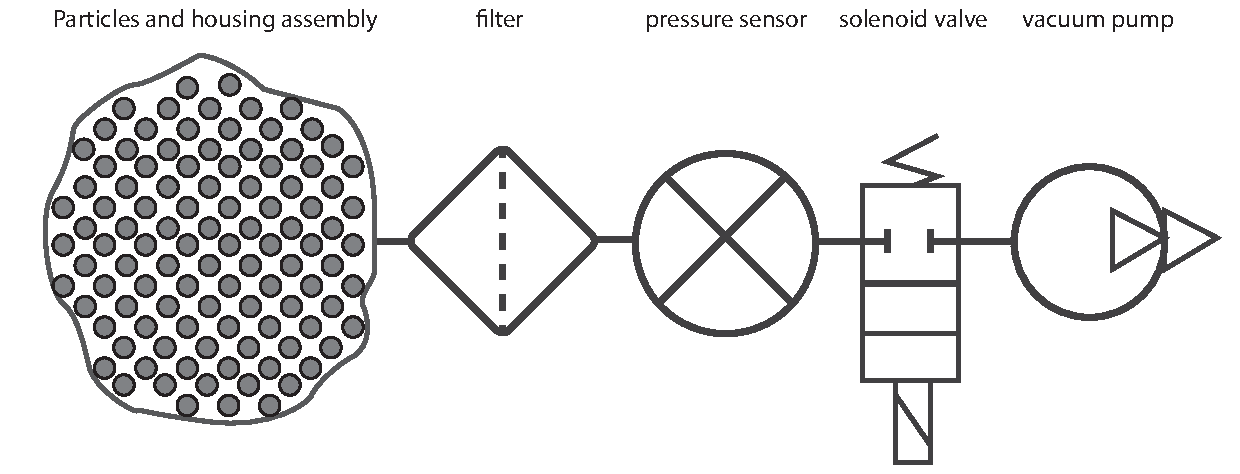
\includegraphics[width=.9\textwidth]{figures/jamming/jamming-basics.pdf}
  \caption{A basic pneumatic jamming system.}
  \label{fig:ch:jamming:jamming-basics}
\end{figure}

Jamming makes it possible to deform an object by hand while in the liquid state and then apply the vacuum and make the deformed object solid - in a sense the form is \emph{saved} as long as the vacuum is maintained.
Figure~\ref{fig:ch:jamming:jamming-transition} shows a transition where a form has been molded and solidified into a shape.
When the pressure is released the form gradually changes shape as seen in the individual steps of the figure.
In this setup we used a balloon as the membrane and ground coffee within as particles.
Pressure was applied with a vacuum cleaner and a coffee filter prevents the particles from being sucked out.
In the example it can be seen that the object (balloon) returns to its initial state which is a requirement for SCIs as stated earlier in section \ref{ch:jamming:vocabulary}.
In this example it is the tension of the rubber latex of the balloon that forces it back but it could as well have been an actuation done with the jamming technique itself. 

\begin{figure}[h]
  \centering
  \includegraphics[width=.9\textwidth]{figures/jamming/jamming-transition}
  \caption[A jamming transition setup.]
  {Jamming transition with a balloon, ground coffee, vacuum cleaner and a coffee filter.}
  \label{fig:ch:jamming:jamming-transition}
\end{figure}

Until now we have talked about jamming as changing stiffness of a single volume, see figure~\ref{fig:ch:jamming:approaches:basic}.
There are examples, which we present in the next section, that apply a more advanced technique with multiple jamming volumes.
In this case a volume is divided into series of cells each of which operate as an individual jamming volume.
The division allows for stiffness control of separate areas on the surface of the entire volume and thus broadens the shape-changing capabilities.
This approach is most often combined with an extra means of actuation to affect the combined volume area typically by pressure by gas or by an inner expanding volume. 
Figure~\ref{fig:ch:jamming:approaches:cell} illustrates the cell-based jamming approach with an inner actuator.
This technique furthermore extends the types of shape-change possible due to its ability to affect the volume by expansion and contraction. 

\begin{figure}
  \centering
  \begin{minipage}[t]{.44\textwidth}
    \centering
    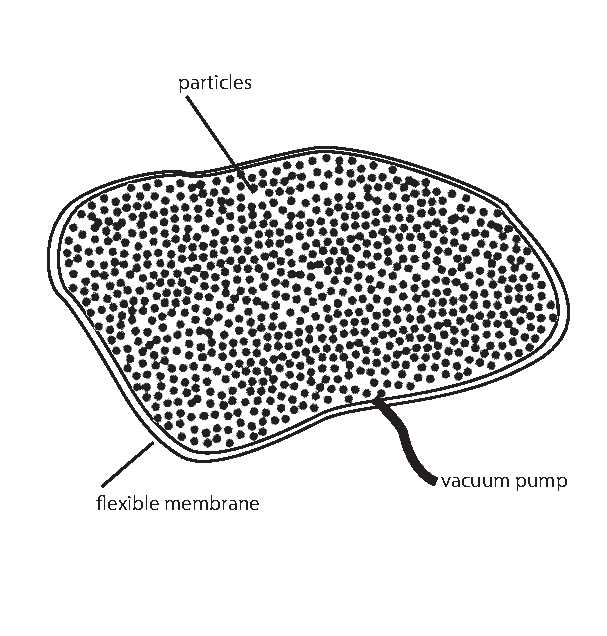
\includegraphics[width=\linewidth]{figures/jamming/basic_jamming}
    \caption[The basic jamming approach.]
    {Illustrates the basic approach with a single jammable volume.}
    \label{fig:ch:jamming:approaches:basic}     
  \end{minipage}
  \hspace{0.02\textwidth}
  \begin{minipage}[t]{.44\textwidth}
    \centering
    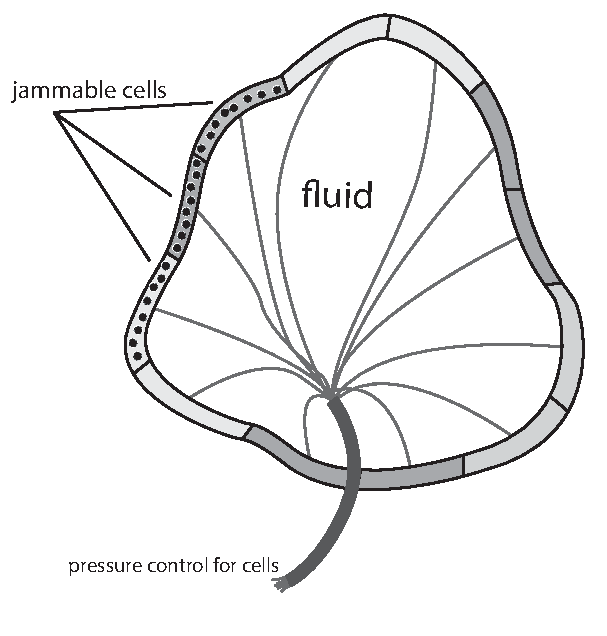
\includegraphics[width=\linewidth]{figures/jamming/cell_jamming}
    \caption[The cell-based jamming approach.]
    {Illustrates the cell-based approach where each cell functions as an independent jammable volume. An inner actuator can contract and expand to control pressure on the cell.}
    \label{fig:ch:jamming:approaches:cell}
  \end{minipage}%
\end{figure}



\section{Related work}
\label{ch:jamming:related-work} 
%!TEX root = ../thesis.tex
Although jamming might seem as a novel approach in the area of HCI, other areas of research have had it on their agenda for some time. 
Especially in the area of mechanical engineering where the jamming mechanism has shown promising results in robotic applications as a substitute for mechanical parts.
In the following we cover the current applications of jamming in both HCI and engineering. 

\subsubsection{Mechanical engineering and robotics}

\citet{brown2010universal, amend2012positive} used the jamming technique to develop a universal robotic gripper \hl{derudover 15,17,18,19 fra referencer i det paper}. 
A gripper is the tool at the end of a robotic arm that interacts with its environment.
This gripper was simply build with an elastic bag as a container for the granular material, which was chosen to be grounded coffee. 
It is able to pick up objects of heterogeneous shapes due to the gripper simply adapting to the surface structure of the objects on impact, see figure~\ref{fig:ch:jamming:jamming-robot-gripper}. 
\todo{this is cool because\dots 1-degree freedom $\rightarrow$ modulated into multi DoF}

\begin{figure}[hb]
	\centering
  		\includegraphics[width=4in]{figures/jamming/jamming-robot-gripper}
	\caption[A universal robotic gripper based on the jamming of granular material by \citet{brown2010universal}.]
   {A universal robotic gripper based on the jamming of granular material.}
   \label{fig:ch:jamming:jamming-robot-gripper}
\end{figure}

Jamming is also seen in experiments with autonomous robots where the mechanism be can used as artificial muscles.

\citet{steltz2009jsel} used the jamming technique to create a platform for shape-changing and mobile robots called JSEL (Jamming Skin Enabled Locomotion).
The soft robot can morph its ``skin'' to create movement of the entire body. 
As opposed to the other applications mentioned this work is based on a division of cells, each of which can be jammed and unjammed to create movement, see figure~\ref{fig:ch:jamming:jsel}. 

\citet{steltz2010jamming} took the JSEL approach further combining the cell-based approach with a linear actuator. 
The assembly combines the contraction and extension capabilities of the linear actuator and modulates this 1-degree of freedom (DoF) actuation into a multi-DoF actuator depending on the number of surrounding jamming cells.
The platform is called JMU (Jamming Modulated Unimorph) and has been tested as component segments of a worm, as an example of a soft robot (see figure~\ref{fig:ch:jamming:jmu}).

These different examples from other fields of research illustrate how creative implementations of the jamming technique and adding other layers of actuation can extend the applicability of jamming.
\todo{purpose $\to$ human unfriendly environments}

\begin{figure}[h]
  \centering
  \begin{minipage}[t]{.45\textwidth}
    \centering
    \includegraphics[width=.9\linewidth]{figures/jamming/chembot-robot-blob}
    \caption[Jamming Skin Enabled Locomotion (JSEL) by \citet{steltz2009jsel}.]
    {Jamming Skin Enabled Locomotion (JSEL). Each cell can be jammed individually to create motion.}
    \label{fig:ch:jamming:jsel}
    \hspace{.2\textwidth} 
  \end{minipage}%
  \hspace{0.5cm}
  \begin{minipage}[t]{.45\textwidth}
    \centering
    \includegraphics[width=.9\linewidth]{figures/jamming/jmu-worm}
    \caption[Jamming Modulated Unimorph by \citet{steltz2010jamming}.]
    {Jamming Modulated Unimorph.}
    \label{fig:ch:jamming:jmu}
  \end{minipage}
\end{figure}

\subsubsection{Human-computer Interaction}
\label{ch:jamming:related-work:hci}
There are only a few research papers published with emphasis on jamming in Human-computer Interaction (HCI). \todo{\dots}
%Table~\ref{ch:jamming:tab:applications_overview} on page \pageref{ch:jamming:tab:applications_overview} shows an overview of the applications mentioned in this section.

\paragraph{The HoverMesh}
\label{ch:jamming:related-work:hci:hovermesh}
\citet{mazzone2004hovermesh} did some early work on creating a deformable structure with the jamming technique. 
The HoverMesh prototype is a cell-based jamming system consisting of 3x3 grid, see figure~\ref{fig:ch:jamming:hovermesh}.
The grid is mounted on top of a cubicle which can be inflated and deflated and together with the grid it creates deformations of the surface structure.
The HoverMesh prototype is not fully implemented according to the ideas presented.
It consists only of the grid structure on top of the cubicle and does not exhibit input capabilities through vision-based techniques and haptic feedback output as intended. 
\todo{A bit of a primitive construction. But }

\paragraph{ClaytricSurface}
\label{ch:jamming:related-work:hci:claytric}
\citet{matoba2012claytricsurface} created a flexible tabletop surface, ClaytricSurface, which serves as a sculptable display medium, see figure~\ref{fig:ch:jamming:claytric-surface}. 
The surface can be directly manipulated by hand and the stiffness can be controlled in real time by a GUI slider.
The exemplified application in this short paper is a painting application projected onto the surface from above and a user can use direct touch on the surface to draw. 
The input is detected by a depth camera from above the tabletop.
\todo{critical points: depth camera and project. and application - 1-page-paper though, it exists in a longer version in Japanese}
\todo{the videos give a more artistic impression of the applicability.}

\begin{figure}[h]
  \centering
  \begin{minipage}[t]{.45\textwidth}
    \centering
    \includegraphics[width=.9\linewidth]{figures/jamming/hovermesh}
    \caption[The HoverMesh by \citet{mazzone2004hovermesh}.]
    {The HoverMesh.}
    \label{fig:ch:jamming:hovermesh}
  \end{minipage}%
  \hspace{0.5cm}
  \begin{minipage}[t]{.45\textwidth}
    \centering
    \includegraphics[width=.9\linewidth]{figures/jamming/claytric-surface}
    \caption[Claytric Surface by \citet{matoba2012claytricsurface}.]
    {Claytric Surface.}
    \label{fig:ch:jamming:claytric-surface}
  \end{minipage}
\end{figure}

\paragraph{Jamming User Interfaces}
\label{ch:jamming:related-work:hci:jui} 
\citet{follmer2012jamming} has probably made the biggest contribution yet to the use of jamming in HCI. 
The authors coin the approach \textit{Jamming User Interfaces} and position it in the area of malleable and organic user interfaces. 
They make several contributions to the field by exploring jamming interfaces for haptic feedback, for malleable tabletops and for mobile devices, see figure~\ref{fig:ch:jamming:jui-collection}. 
They also investigate how sensing techniques like capacitive and optical sensing, can broaden the applicability of jamming in HCI. 

\citet{follmer2012jamming} also present a hydraulic jamming system that is fast and silent and which allow for transparent jamming volumes. 
This requires transparent particles and a transparent fluid that matches the refractive index of the particles so that light refraction is reduced. 
\todo{maybe an image here}

\todo{critical points: very much proof on concept, misses real world implementations.}

In the following we will give a brief overview of the four prototypes implemented and described by \citet{follmer2012jamming}.

\subparagraph{Tunable Clay} is a malleable tabletop for direct 3D modelling, see figure~\ref{fig:ch:jamming:jui-clay}
It resembles ClaytricSurface \citep{matoba2012claytricsurface} mentioned earlier with is clay-like surface that can easily be deformed.
Tunable Clay uses the hydraulic jamming system mentioned above with index-matched particles and fluid.
This allows for a more sophisticated depth sensing approach than the one used with ClaytricSurface.
Optical shape sensing and graphic projection is integrated underneath the jamming volume.
The shape, captured in real-time, is shown as a virtual 3D model on both an external display and on the jamming volume itself projected from underneath the surface.

\subparagraph{Transparent Haptic Lens} is small tangible puck to be used as a haptic information channel on a tabletop display, see figure~\ref{fig:ch:jamming:jui-lens}.
It has a transparent lens in the center which is a transparent hydraulic jamming volume which can change its stiffness according to the texture beneath it.
A user presses \todo{a/his/hers} finger into the lens to get a haptic sensation about the underlying texture of the image directly underneath. 

\subparagraph{Behind-the-Tablet Jamming} is a tablet computer which has a pneumatic jamming volume mounted on the backside, see figure~\ref{fig:ch:jamming:jui-tablet}.
The system senses malleable input with capacitive shape sensing.
The scenarios envisioned are for navigating content (e.g. scrolling and zooming) on the tablet display through malleable interaction on the backside. 
The system can communicate that some limit is reached with haptic feedback, 
e.g. by stiffening the jamming volume.

\subparagraph{ShapePhone} is a generic mobile device that can be shaped and locked into different forms, see figure~\ref{fig:ch:jamming:jui-phone}.
The device has no technology inside, except for the jamming system, and it merely serves as demonstration of how its affordances change when it is sculpted into forms resembling e.g. a phone, remote control or a watch.
Ideas are presented for integrating various sensing techniques such as capacitive shape sensing and touch sensing to derive contextual information.

\begin{figure}
        \centering
        \begin{subfigure}[b]{0.45\textwidth}
                \centering
                \includegraphics[width=\textwidth]{figures/jamming/jui_tunable-clay}
                \caption{Tuneable Clay}
                \label{fig:ch:jamming:jui-clay}
        \end{subfigure}
        \begin{subfigure}[b]{0.45\textwidth}
                \centering
                \includegraphics[width=\textwidth]{figures/jamming/jui_haptic-lens}
                \caption{Transparent Haptic Lens}
                \label{fig:ch:jamming:jui-lens}
        \end{subfigure}

        \begin{subfigure}[b]{0.45\textwidth}
                \centering
                \includegraphics[width=\textwidth]{figures/jamming/jui_behind-the-tablet}
                \caption{Behind-the-Tablet Jamming}
                \label{fig:ch:jamming:jui-tablet}
        \end{subfigure}
        \begin{subfigure}[b]{0.45\textwidth}
                \centering
                \includegraphics[width=\textwidth]{figures/jamming/jui_shapephone}
                \caption{ShapePhone}
                \label{fig:ch:jamming:jui-phone}
        \end{subfigure}
        \caption{Jamming User Interfaces by \citet{follmer2012jamming}.}
        \label{fig:ch:jamming:jui-collection}
\end{figure}

\subsection{Summary}

In the previous sections we have given an introduction to the mechanics of jamming and an overview of different research applications of jamming.
Table \ref{ch:jamming:table:applications_overview} summarises and categorises these applications according to their characteristics.
In the next we will move on to our own concepts that support the notion of ad hoc interfaces.

\begin{landscape}
  \thispagestyle{empty}
  \centering
  \captionof{table}{An overview of jamming in HCI} \label{ch:jamming:table:applications_overview} 
  \begin{tabularx}{\linewidth}{|l|c|c|c|c|c|X|}
    \hline
    Project & Input & Output & Type & Particles & Transparent & Summary \\ \hline
    The HoverMesh & \cellcolor{FalseColor}\xmark & \cellcolor{TrueColor}\cmark & pneumatic & polystyrene (2-3 mm) & \xmark & A cell-based deformable surface structure . \\ \hline    
    ClaytricSurface & \cellcolor{TrueColor}\cmark & \cellcolor{FalseColor}\xmark & pneumatic & polystyrene & \xmark & A flexible tabletop surface which serves as a sculptable display medium. \\ \hline
      Tunable Clay & \cellcolor{TrueColor}\cmark & \cellcolor{FalseColor}\xmark & hydraulic & glass beads & \cmark & A malleable tabletop for direct 3D modelling. \\ \hline
      Transparent Haptic Lens & \cellcolor{FalseColor}\xmark & \cellcolor{TrueColor}\cmark & hydraulic & glass beads & \cmark & A small tangible puck to be used as a haptic information channel on a tabletop display. \\ \hline
      Behind-the-Tablet Jamming & \cellcolor{TrueColor}\cmark & \cellcolor{TrueColor}\cmark & pneumatic & ? & \xmark & A tablet with a interactive jamming volume on the back. \\ \hline
      ShapePhone & \cellcolor{TrueColor}\cmark & \cellcolor{FalseColor}\xmark & pneumatic & coffee (coarse or fine ?) & \xmark & a generic mobile device that can be shaped and locked into different forms. \\
      \hline
  \end{tabularx}

\begin{flushleft}
This table is an overview of the prototypes presented in the papers covered in this section. It should be mentioned that in categorising \textit{input} and \textit{output} features we are only considering whether input or output is enabled using the jamming technique. For example, \textit{Tunable Clay} does have output in the form a image projection but it does not utilise the jamming technique.
\todo{information is of course retrieved from the papers but some parts are not available. Check other sources: web pages, videos, email author??}
\end{flushleft}

\end{landscape}


\section{Concepts}
\label{ch:jamming:concepts} 
%!TEX root = ../thesis.tex
This section will focus on describing and discussing a selection of concepts for ad hoc interfaces based the jamming technique.
As mentioned in the beginning of this chapter we were not succesfull at implementing a working jamming system where we could control air/liquid flow. \todo{make sure this is actually adressed. Suggestions: complexity, price of equipment: mechanics is one thing, the other is materials, i.e. ecoflex rubber etc.}
Therefore we concentrate on conceptual prototypes which we envisioned before taking the descision to move in other directions.

\subsection{(Car) dashboard} 

\todo{what's the problem with static (car) dashboards}\\

Cell-based jamming as mentioned in \ref{ch:jamming} allows for deformations of individual cells.
This technique \hl{opens up} for a new and very dynamic approach to inputs, such as buttons, knobs, etc.
These input controls could emerge from the otherwise flat surface when needed, see figure~\ref{fig:ch:jamming:concepts:button} 

\begin{figure}[h]
  \centering
      \includegraphics[width=3in]{figures/jamming/concepts/button}
  \caption[A cell-based jammable button.]
  {A cell-based jammable button.}
  \label{fig:ch:jamming:concepts:button}
\end{figure}




\section{Technicalities}
\section{Discussion}
\todo{Maybe some Gaver (research through design) and (Alternatives, conceptual design proposals )}